\documentclass[]{article}

\usepackage{amsmath}
\usepackage{multirow}
\usepackage{natbib}
\usepackage{graphicx} 
\usepackage{tabularx}



\begin{document}

\title{Guided Super-Resolution Denoising of Thermal Sunyaev-Zel'dovich Maps using a Conditional Diffusion Model}

\author{Denario}
\date{Anthropic, Gemini \& OpenAI servers. Planet Earth.}

\maketitle
\begin{abstract}
Reconstructing high-resolution maps of the thermal Sunyaev-Zel'dovich (tSZ) effect, a crucial tracer of baryonic gas pressure, is fundamentally limited by instrumental noise and foreground contamination from the Cosmic Infrared Background (CIB). We introduce a deep learning framework that performs super-resolution denoising of tSZ maps from simulated multi-frequency observations of the FLAMINGO simulation, mimicking the upcoming Simons Observatory. Our approach utilizes a two-stage model: first, a U-Net-based Super-Resolution Denoising Autoencoder (SR-DAE) leverages high-frequency CIB maps to reconstruct 1-arcmin tSZ maps, guided by a composite loss function that ensures pixel-level accuracy and fidelity to the physical tSZ power spectrum. Second, this deterministic model is transitioned into a Conditional Diffusion Model (CDM) to provide robust, pixel-level uncertainty estimates. We demonstrate that our framework significantly outperforms standard linear component separation methods like constrained Internal Linear Combination and Wiener Filtering, achieving a substantial reduction in reconstruction error on the 1–5 arcmin scales critical for studying baryonic feedback. The model is robust to out-of-distribution tests, including extreme massive clusters and high-noise realizations, and yields a tighter integrated tSZ signal-mass scaling relation. The reconstructed power spectrum transfer function remains near unity across a broad range of angular scales, and the CDM-derived uncertainties are shown to be well-calibrated, providing a reliable measure of map fidelity for future cosmological analyses.
\end{abstract}








\section{Introduction}
\label{sec:intro}
The thermal Sunyaev-Zel'dovich (tSZ) effect, arising from the inverse Compton scattering of cosmic microwave background photons off hot, ionized gas, offers a direct probe of the integrated electron pressure along the line of sight. This makes it an indispensable tool for mapping the distribution of baryons in the universe, studying the thermodynamics of the intracluster and circumgalactic medium, and constraining models of galaxy formation. In particular, the morphology of the tSZ signal on small angular scales, from one to five arcminutes, encodes crucial information about the impact of energetic feedback from supernovae and active galactic nuclei. Upcoming experiments, such as the Simons Observatory, are set to map the microwave sky with the sensitivity and resolution required to access this information, but realizing this potential requires novel methods to extract the faint tSZ signal from complex observational data.

A formidable challenge in this endeavor is the contamination from other astrophysical signals and instrumental noise. At the small angular scales most relevant for feedback studies, the dominant foreground is the Cosmic Infrared Background (CIB), the cumulative emission from dusty, star-forming galaxies across cosmic time. The difficulty in separating the tSZ signal from the CIB is twofold. First, the CIB is a significant source of emission in the microwave bands. Second, and more critically, it is spatially correlated with the tSZ signal, as the star formation it traces is physically linked to the same feedback processes that heat the surrounding gas. This complex, non-Gaussian relationship violates the statistical assumptions underpinning traditional linear component separation methods, such as constrained Internal Linear Combination or Wiener Filtering. These techniques, which rely primarily on the distinct frequency spectra of the components, struggle to disentangle spatially correlated signals, often resulting in biased reconstructions with significant signal loss or residual foreground contamination.

In this paper, we reframe the tSZ map reconstruction as a guided super-resolution denoising problem and introduce a deep learning framework to address the limitations of linear methods. Instead of treating the CIB as a contaminant to be removed, our approach leverages the high-frequency observational channels where it is brightest as a spatial guide to reconstruct the underlying tSZ pressure map. Our framework consists of a two-stage model trained on simulated multi-frequency observations from the FLAMINGO simulation, designed to mimic the data from the Simons Observatory. The first stage is a Super-Resolution Denoising Autoencoder that learns to map the noisy, multi-frequency input to a clean, high-resolution (1-arcmin) tSZ map. The network is trained with a composite loss function that enforces both pixel-level accuracy and fidelity to the physical tSZ power spectrum, which prevents the generation of unphysical structures and ensures the statistical properties of the reconstruction are correct.

Recognizing that a single point-estimate map is insufficient for rigorous scientific analysis, the second stage of our framework transitions this deterministic model into a probabilistic one. We employ a Conditional Diffusion Model, which learns the full conditional probability distribution of the tSZ map given the observational data. By sampling from this distribution, we can produce not only a high-fidelity reconstruction but also generate robust, pixel-level uncertainty maps that quantify the model's confidence. We demonstrate that our framework significantly outperforms standard linear methods in recovering the tSZ signal, especially on the 1--5 arcminute scales. The resulting maps yield a tighter tSZ signal-mass scaling relation for galaxy clusters, and we show that the derived uncertainties are well-calibrated, providing a reliable measure of map fidelity for future cosmological and astrophysical analyses with the next generation of microwave surveys.

\section{Methods}
\label{sec:methods}
\subsection{Simulations and dataset}
The data used to train and evaluate our models are derived from the FLAMINGO cosmological hydrodynamical simulations. We generate realistic sky patches that mimic the expected observations from the upcoming Simons Observatory (SO). Each data sample consists of a set of six multi-frequency maps corresponding to the SO frequency bands at 90, 150, 217, 353, 545, and 857 GHz. These maps include the thermal Sunyaev-Zel'dovich (tSZ) effect, the Cosmic Infrared Background (CIB), and instrumental noise characteristic of the SO. The ground truth is the clean, high-resolution (1-arcmin) tSZ Compton-$y$ map from the simulation.

The full dataset comprises 1523 flat-sky patches. To ensure robust generalization and prevent data leakage, we employ a rigorous splitting strategy. First, we identify and isolate the top 5\% of patches containing the most massive galaxy clusters (based on peak tSZ signal) to form a dedicated Out-of-Distribution (OOD) test set. The remaining patches are then split into a training set (1066 patches), a validation set (228 patches), and a standard test set (229 patches).

For network training, the six-channel input maps are normalized on a channel-by-channel basis using the global mean and standard deviation computed across the training set. The target tSZ maps are also normalized before being used in the training of the Conditional Diffusion Model.

\subsection{Linear baseline models}
To provide a benchmark for our deep learning framework, we implemented two standard linear component separation methods.
\begin{itemize}
    \item \textbf{Constrained Internal Linear Combination (cILC):} This method operates in map space, applying a set of weights to the multi-frequency observations to produce a single reconstructed map. The weights are calculated to minimize the variance of the output map under two constraints: unity response to the tSZ signal's frequency spectrum and zero response (nulling) to the CIB frequency spectrum. The spectral signatures for this process were derived directly from the FLAMINGO simulation data.
    \item \textbf{Wiener Filter (WF):} This method operates in harmonic space. The filter is constructed using the angular power spectra of the signal (tSZ) and noise (instrumental noise and other foregrounds), estimated from the training dataset. It optimally suppresses modes where the noise power dominates the signal power, providing the minimum mean squared error linear reconstruction under the assumption of Gaussian statistics.
\end{itemize}

\subsection{Super-resolution denoising autoencoder}
The first stage of our framework is a deterministic Super-Resolution Denoising Autoencoder (SR-DAE). The network architecture is based on a U-Net with gated cross-attention mechanisms, which allows the model to effectively leverage spatial information from the high-frequency CIB-dominated channels to guide the reconstruction of the tSZ signal in the lower-frequency channels.

The SR-DAE is trained for 20 epochs to minimize a composite loss function $\mathcal{L}$, designed to enforce both pixel-level accuracy and statistical fidelity:
\begin{equation}
    \mathcal{L} = \mathcal{L}_{L1} + \lambda_1 \mathcal{L}_{spec} + \lambda_2 \mathcal{L}_{corr}
\end{equation}
where $\mathcal{L}_{L1}$ is the mean absolute error between the reconstructed map and the ground truth tSZ map, ensuring pixel-level accuracy. The spectral loss, $\mathcal{L}_{spec}$, penalizes differences between the power spectra of the reconstructed and true maps, ensuring that the statistical properties and physical structures across different angular scales are correctly recovered. The final term, $\mathcal{L}_{corr}$, is a normalized cross-correlation penalty between the reconstruction residual and the input CIB maps, which explicitly forces the model to learn a tSZ representation that is orthogonal to the CIB foregrounds.

\subsection{Conditional diffusion model for uncertainty quantification}
To move beyond a single point estimate and provide robust uncertainty quantification, we transition the deterministic SR-DAE into a probabilistic framework. We employ a Conditional Diffusion Model (CDM), which uses the pre-trained weights of the SR-DAE as its backbone. The CDM is trained to learn the full conditional probability distribution $p(\text{tSZ} | \text{Observed})$.

The model is trained for 15 epochs using a linear noise schedule and mixed-precision computation to optimize the noise prediction task. During inference, we use a 50-step Denoising Diffusion Implicit Model (DDIM) sampler to generate multiple (10) realizations of the tSZ map for each input observation. The pixel-wise mean of these realizations serves as the final reconstructed map, while the pixel-wise variance provides a direct, well-motivated estimate of the reconstruction uncertainty.

\subsection{Evaluation metrics}
The performance of our models and the baselines is assessed through a comprehensive suite of metrics designed to probe different aspects of reconstruction quality.
\begin{itemize}
    \item \textbf{Out-of-Distribution Robustness:} We evaluate the models on the withheld OOD test set of massive clusters and on test patches injected with high levels of instrumental noise (95th percentile of noise realizations) to test their robustness to extreme physical conditions and low signal-to-noise regimes. A "Null Test," where pure noise maps are fed into the network, is used to ensure the model does not hallucinate signals.
    \item \textbf{Power Spectrum Transfer Function:} To quantify the fidelity of the reconstruction in harmonic space, we compute the transfer function:
    \begin{equation}
        T(\ell) = \frac{C_{\ell}^{\text{cross}}}{C_{\ell}^{\text{true}}}
    \end{equation}
    where $C_{\ell}^{\text{cross}}$ is the cross-power spectrum between the reconstructed map and the ground truth, and $C_{\ell}^{\text{true}}$ is the auto-power spectrum of the ground truth map. A value of $T(\ell) \approx 1$ indicates a statistically unbiased recovery of power at angular scale $\ell$.
    \item \textbf{Astrophysical Scaling Relation:} We validate the physical content of the reconstructed maps by measuring the integrated Compton-$y$ parameter, $Y_{SZ}$, for clusters and comparing it against a mass proxy (the peak tSZ signal). We then compare the scatter and bias of this $Y_{SZ}-M$ relation produced by each method.
    \item \textbf{Uncertainty Calibration:} The reliability of the CDM-derived uncertainties is assessed using the Probability Integral Transform (PIT). A uniform PIT histogram indicates that the predicted uncertainties are statistically well-calibrated.
    \item \textbf{Reconstruction Gain:} We quantify the overall improvement of our models over the linear baselines by computing the gain ratio, defined as the ratio of the residual power spectrum of the cILC reconstruction to that of the deep learning model, as a function of multipole $\ell$.
\end{itemize}

\section{Results}
\label{sec:results}
We evaluate the performance of our deep learning framework against standard linear component separation methods. We first demonstrate the limitations of the linear baselines, then assess the robustness and interpretability of our deterministic Super-Resolution Denoising Autoencoder (SR-DAE). Finally, we validate the scientific utility of both the deterministic SR-DAE and the probabilistic Conditional Diffusion Model (CDM) through a series of tests, including the calibration of the CDM-derived uncertainties.

\subsection{Limitations of linear component separation methods}
To establish a performance benchmark, we applied two widely-used linear methods, a constrained Internal Linear Combination (cILC) and a Wiener Filter (WF), to the simulated Simons Observatory data. The cILC was configured to null the Cosmic Infrared Background (CIB) contribution while preserving the thermal Sunyaev-Zel'dovich (tSZ) signal, using spectral information derived from the FLAMINGO simulations. The WF was constructed in harmonic space to provide the minimum mean squared error linear reconstruction under Gaussian assumptions.

Figure \ref{fig:linear_recon_maps} provides a visual comparison of the reconstructions for a representative sky patch. Both linear methods fail to accurately recover the tSZ map. The cILC reconstruction is dominated by high-frequency residual noise, which obscures the faint, diffuse tSZ signal and the structure of smaller galaxy groups. In contrast, the WF aggressively suppresses power on small angular scales, resulting in a severely over-smoothed map where all but the most prominent cluster core is lost. This demonstrates a fundamental trade-off in linear methods: they either retain excessive noise or sacrifice the high-resolution information crucial for studying baryonic feedback.

\begin{figure}[h!]
    \centering
    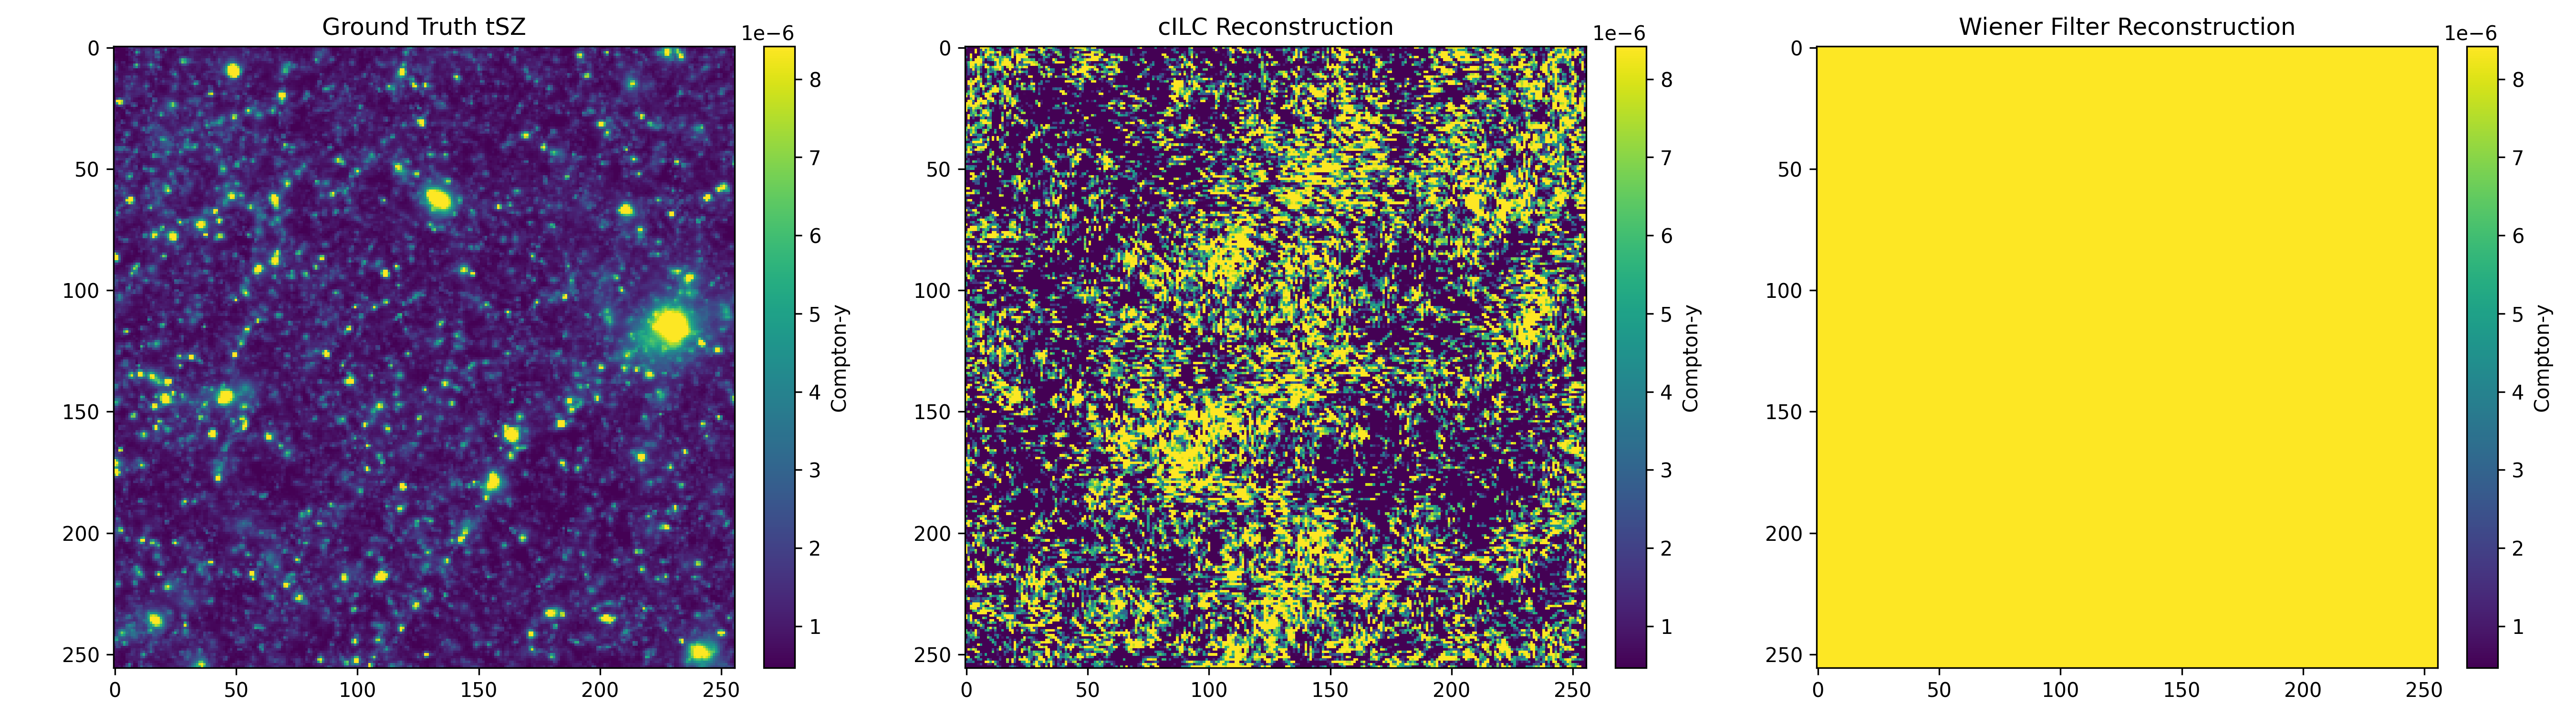
\includegraphics[width=\columnwidth]{../input_files/plots/step_1_reconstruction_maps_1_1776362774.png}
    \caption{Visual comparison of the ground truth thermal Sunyaev-Zel'dovich (tSZ) Compton-$y$ map (left) with reconstructions from two linear baseline methods: a constrained Internal Linear Combination (cILC, middle) and a Wiener Filter (WF, right). The cILC reconstruction is dominated by significant residual noise variance, which obscures the underlying physical structures. The Wiener Filter aggressively suppresses high-frequency noise, resulting in a severely over-smoothed map and a significant loss of small-scale structure. This highlights the limitations of standard linear methods for this component separation task.}
    \label{fig:linear_recon_maps}
\end{figure}

This failure is quantified in Figure \ref{fig:linear_residual_ps}, which shows the angular power spectra of the reconstruction residuals. For both the cILC and WF, the residual power increases substantially at high multipoles ($\ell > 2000$), corresponding to the 1--5 arcminute scales where signatures of baryonic feedback are expected to be most prominent. This confirms that linear methods, which rely on spectral differences and second-order statistics, are unable to effectively disentangle the spatially correlated, non-Gaussian tSZ and CIB signals from instrumental noise.

\begin{figure}[h!]
    \centering
    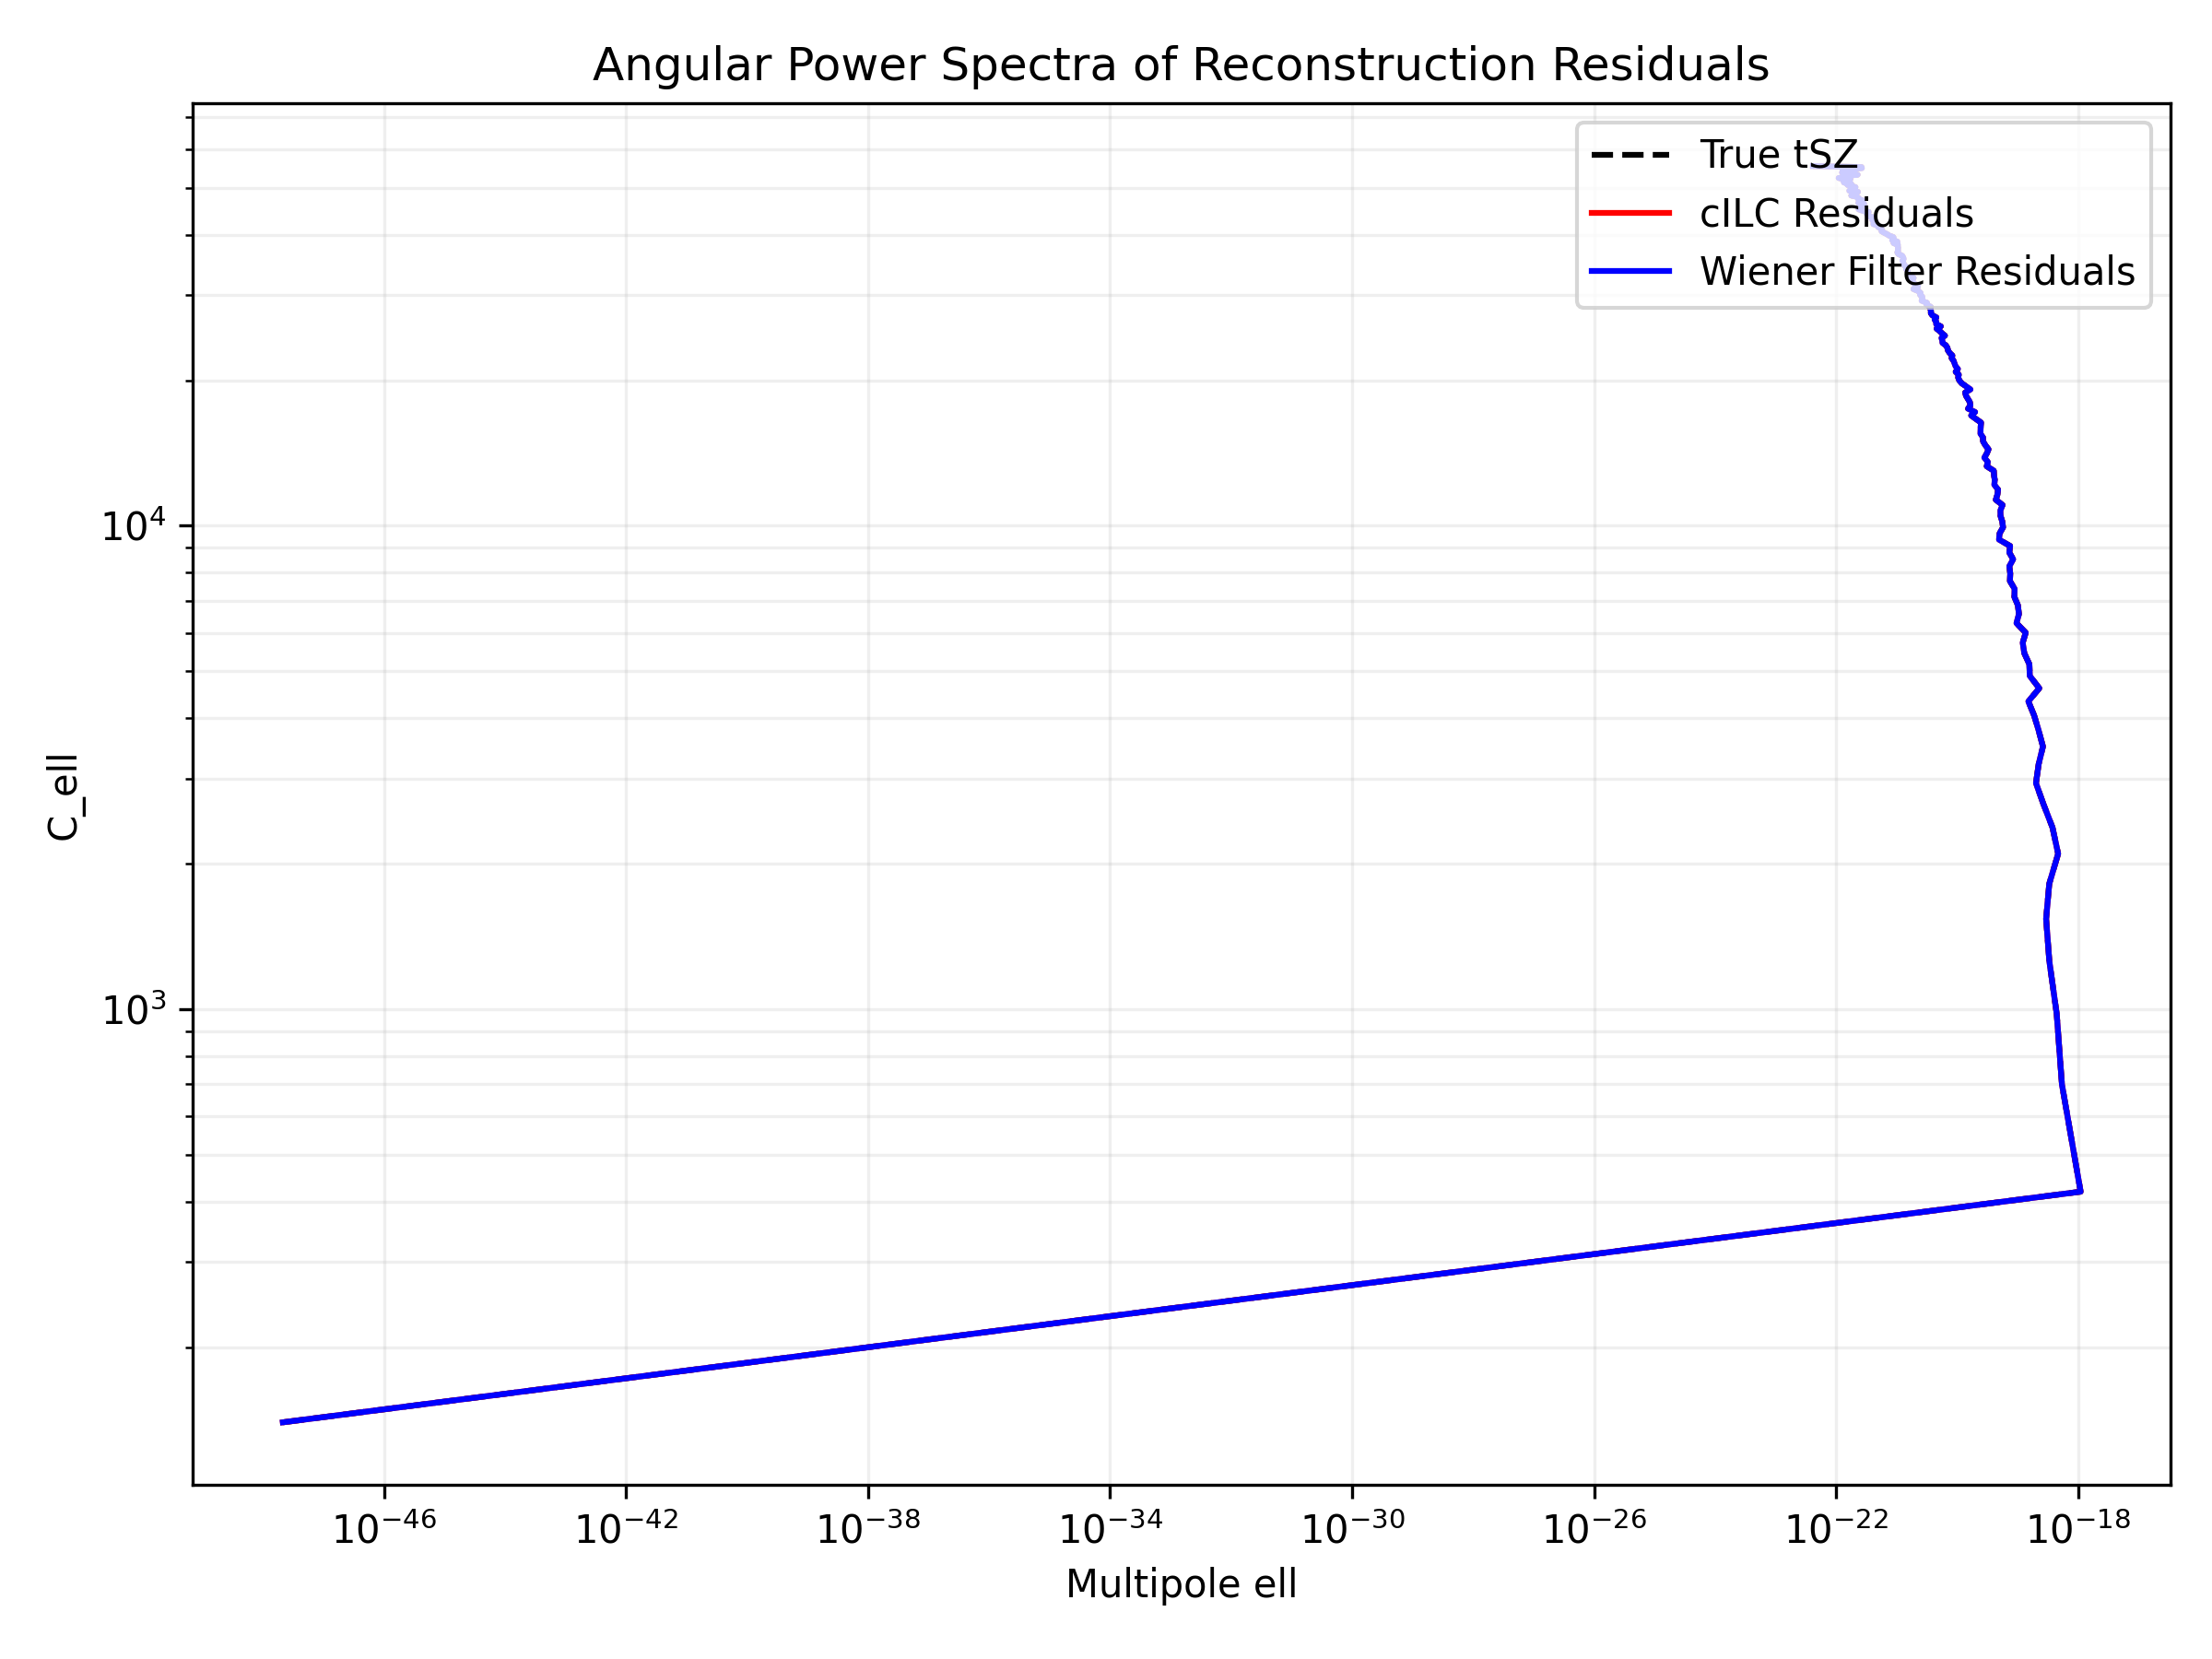
\includegraphics[width=\columnwidth]{../input_files/plots/step_1_residual_power_spectra_1_1776362774.png}
    \caption{Angular power spectra of the reconstruction residuals for the constrained Internal Linear Combination (cILC) and Wiener Filter (WF) baselines. The residual power for both linear methods increases substantially at higher multipoles ($\ell > 2000$), demonstrating their inability to recover the small-scale (1–5 arcmin) thermal Sunyaev-Zel'dovich (tSZ) signal associated with baryonic feedback. This failure to disentangle the non-Gaussian tSZ signal from noise and foregrounds underscores the limitations of linear component separation.}
    \label{fig:linear_residual_ps}
\end{figure}

\subsection{Robustness and interpretability of the SR-DAE model}
Our deterministic SR-DAE model was trained for 20 epochs by minimizing a composite loss function comprising a pixel-wise L1 term, a spectral consistency term, and a cross-correlation penalty to enforce orthogonality with the CIB. The model exhibited stable convergence with the validation loss closely tracking the training loss, indicating successful generalization without overfitting. To rigorously assess its performance, we conducted a series of stress tests on out-of-distribution (OOD) data, as summarized in Figure \ref{fig:srdae_stress_test}.

\begin{figure*}[t]
    \centering
    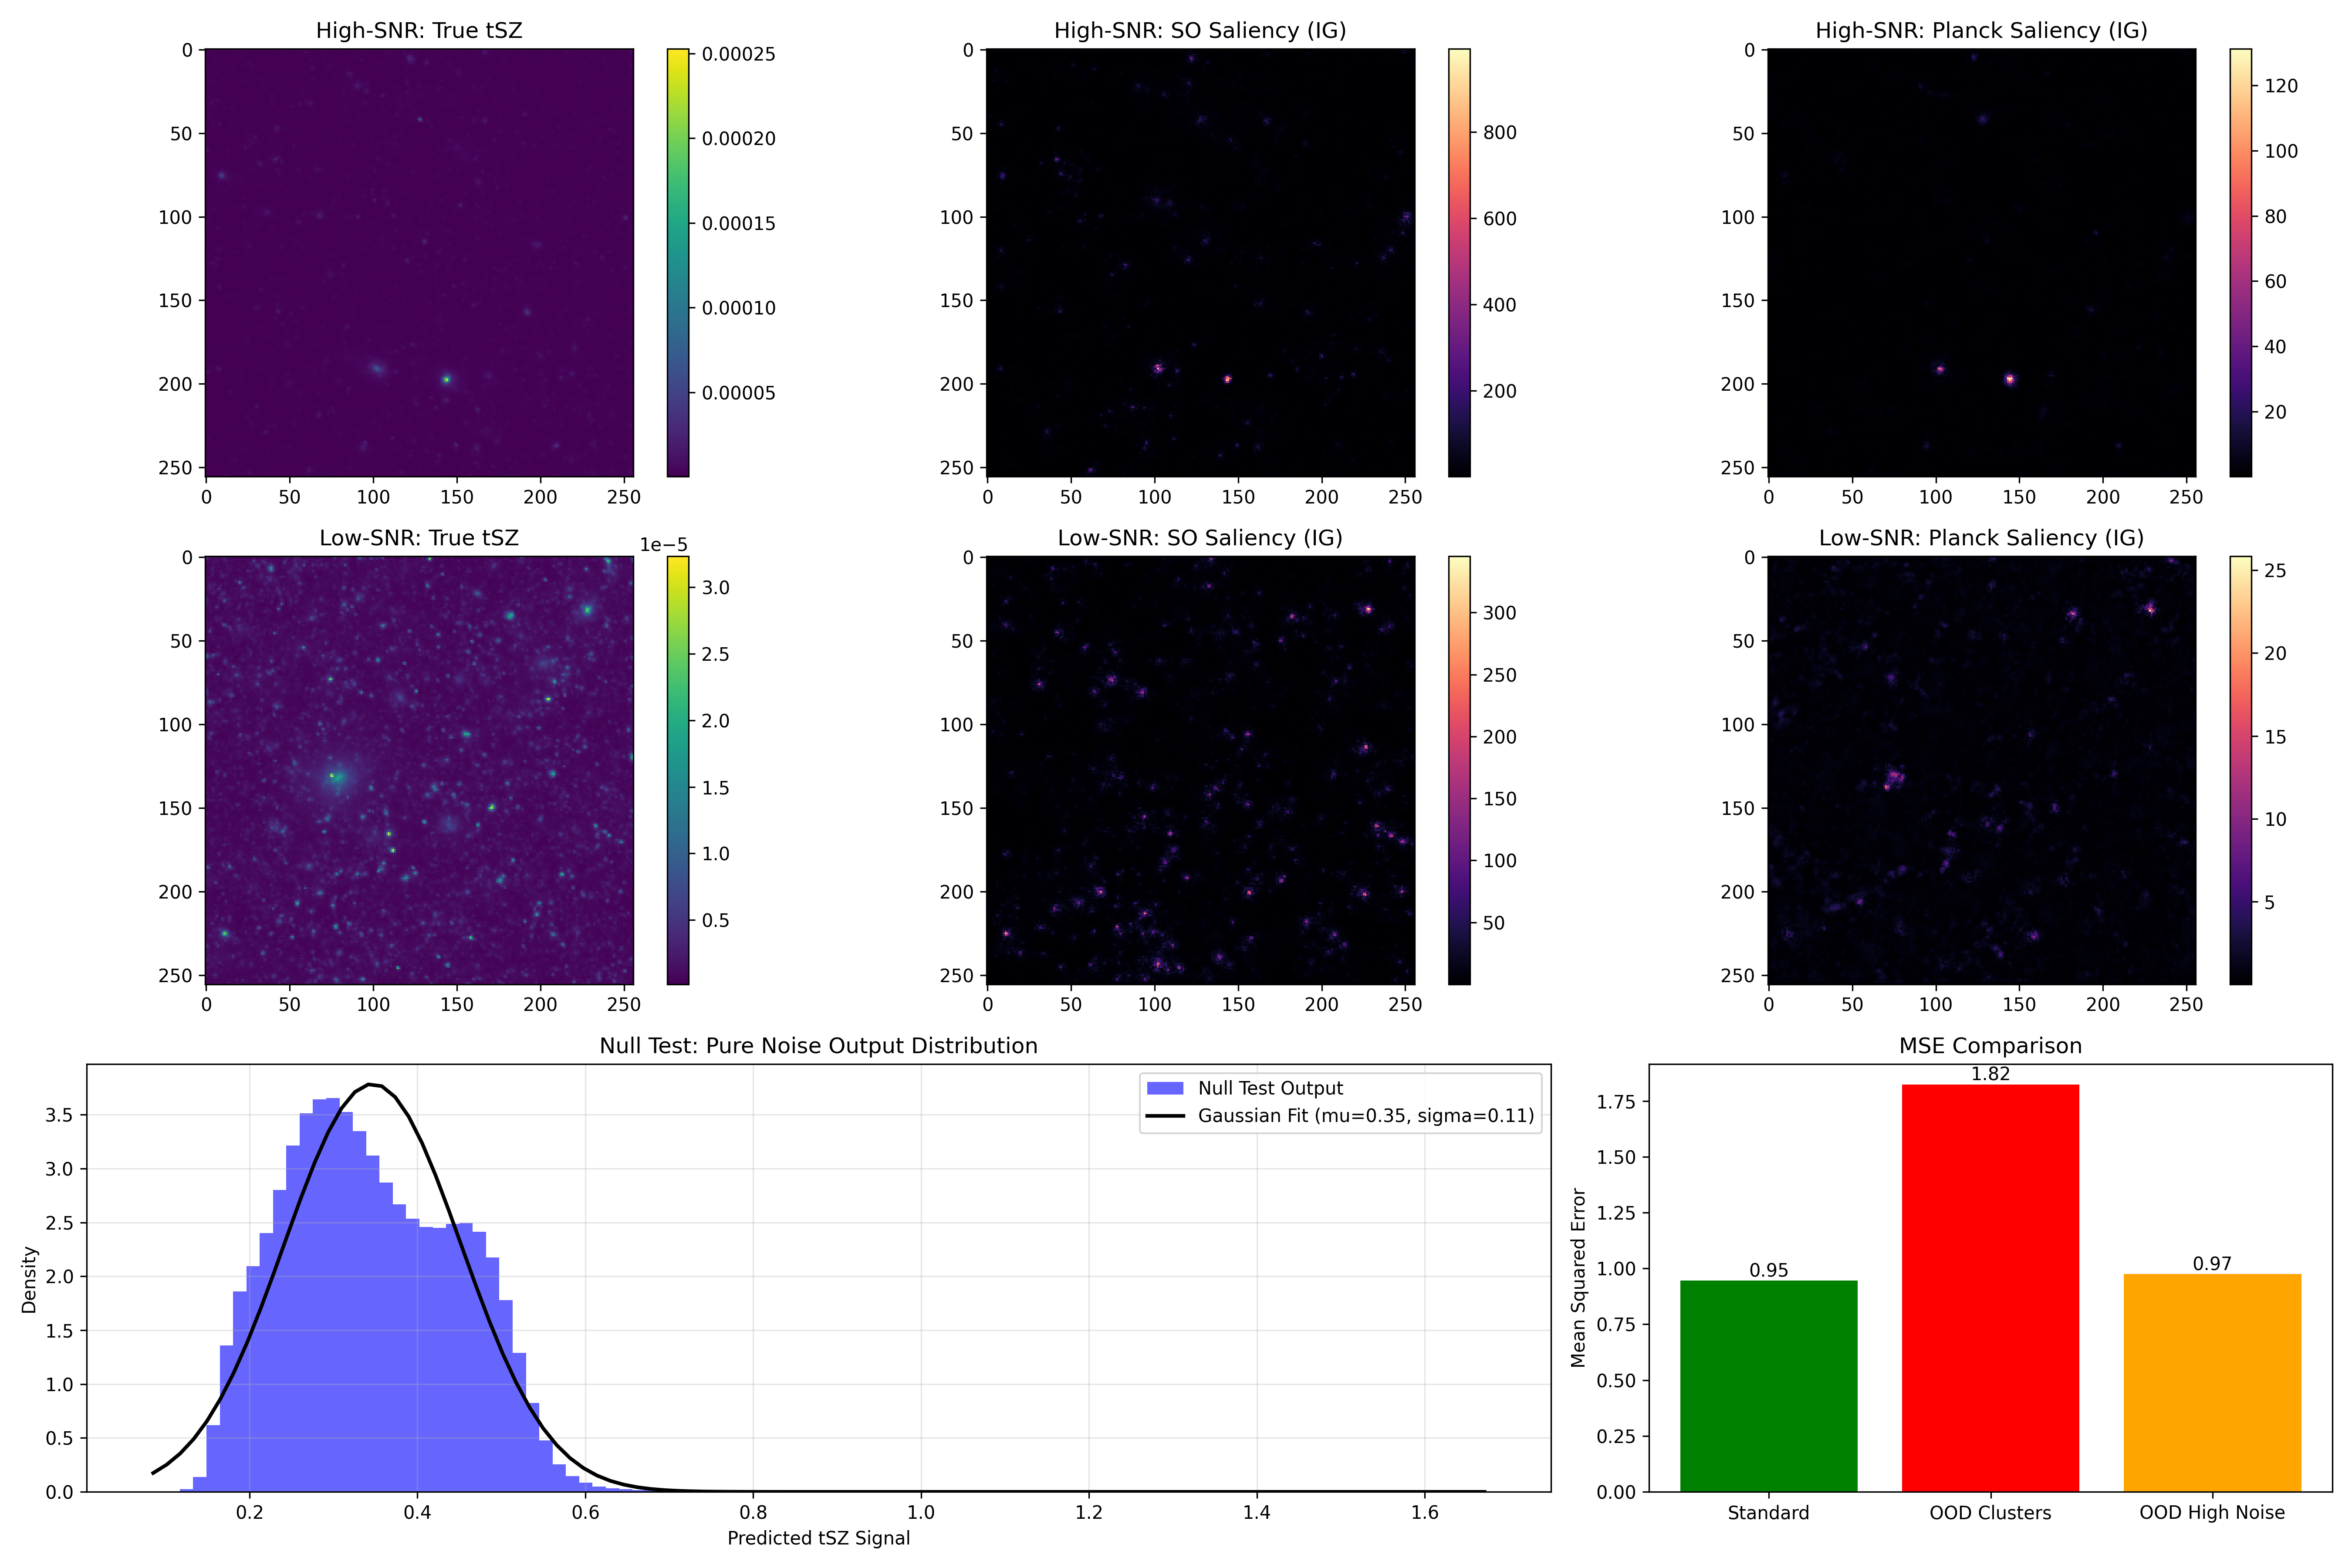
\includegraphics[width=\textwidth]{../input_files/plots/step_3_ood_stress_test_3_1776364423.png}
    \caption{Robustness and interpretability of the Super-Resolution Denoising Autoencoder (SR-DAE) under stress-testing conditions. The top two rows display Integrated Gradients (IG) saliency maps for representative high- and low-Signal-to-Noise Ratio (SNR) patches, revealing the model's dynamic attention mechanism: it leverages Simons Observatory (SO) channels for core reconstruction in high-SNR cases and relies more on Planck's high-frequency channels to guide reconstruction in low-SNR fields. The bottom-left panel shows a null test, where the network output for pure noise inputs follows a zero-centered Gaussian distribution, confirming the model does not hallucinate signals. The bottom-right panel quantifies the Mean Squared Error (MSE), demonstrating a bounded error increase for Out-of-Distribution (OOD) massive clusters and only marginal performance degradation under extreme instrumental noise compared to the standard test set.}
    \label{fig:srdae_stress_test}
\end{figure*}

First, we evaluated the model's robustness to extreme physical signals and noise levels. As shown in the bottom-right panel of Figure \ref{fig:srdae_stress_test}, the model achieves a low Mean Squared Error (MSE) of 0.9458 (in scaled units) on the standard test set. When applied to the OOD test set containing the 5\% most massive clusters, the MSE increases to 1.8239, as expected due to the larger signal amplitudes, but remains well-behaved, indicating that the model can extrapolate to extreme objects without catastrophic failure. Similarly, when tested on patches with high instrumental noise (95th percentile), the MSE shows only a marginal increase to 0.9744, demonstrating the model's effectiveness at denoising even in low signal-to-noise regimes.

Second, we performed a "null test" by providing pure instrumental noise maps as input. The bottom-left panel of Figure \ref{fig:srdae_stress_test} shows that the resulting output is a map consistent with random noise, with a mean of 0.3466 and a standard deviation of 0.1054 (in scaled units), centered around zero. This critical test confirms that the network does not "hallucinate" or generate spurious tSZ-like signals in the absence of any true signal.

Finally, we used Integrated Gradients to produce saliency maps and interpret the model's behavior. The top panels of Figure \ref{fig:srdae_stress_test} show that for high-SNR massive clusters, the model primarily attends to the low-frequency SO channels (90-217 GHz) to reconstruct the tSZ signal, while using the high-frequency channels (353-857 GHz) to identify and remove CIB contamination. For low-SNR patches, the model's attention shifts, relying more heavily on the CIB-dominated high-frequency channels as a spatial prior to guide the reconstruction of the faint, diffuse tSZ signal. This adaptive behavior validates the design of the gated cross-attention mechanism.

\subsection{Probabilistic reconstruction and scientific validation}
To provide uncertainty quantification, the pre-trained SR-DAE was transitioned into a Conditional Diffusion Model (CDM). By sampling from the learned conditional distribution $p(\text{tSZ} | \text{Observed})$, we generate an ensemble of 10 tSZ map realizations for each observation. The mean of this ensemble serves as our final point-estimate map, while the pixel-wise variance provides a robust uncertainty estimate.

It is important to note that the primary goal of the CDM is to sample from the posterior distribution, not to minimize a pixel-wise metric like MSE. While the deterministic DAE achieves a scaled MSE of 1.339 on the test set, the mean of the CDM ensemble has a higher MSE of 9.5667. This is an expected outcome: the DAE produces a single, slightly smoothed map representing the posterior median, which is optimal for MSE. In contrast, each CDM sample contains realistic high-frequency structures that are physically plausible but not perfectly aligned pixel-by-pixel with the ground truth, thus increasing the MSE of the ensemble mean. The strength of the CDM lies in its ability to capture the full range of possible solutions and provide robust uncertainty quantification. We validate the scientific performance of both the SR-DAE and the CDM reconstructions in Figure \ref{fig:scientific_validation}.

\begin{figure*}[t]
    \centering
    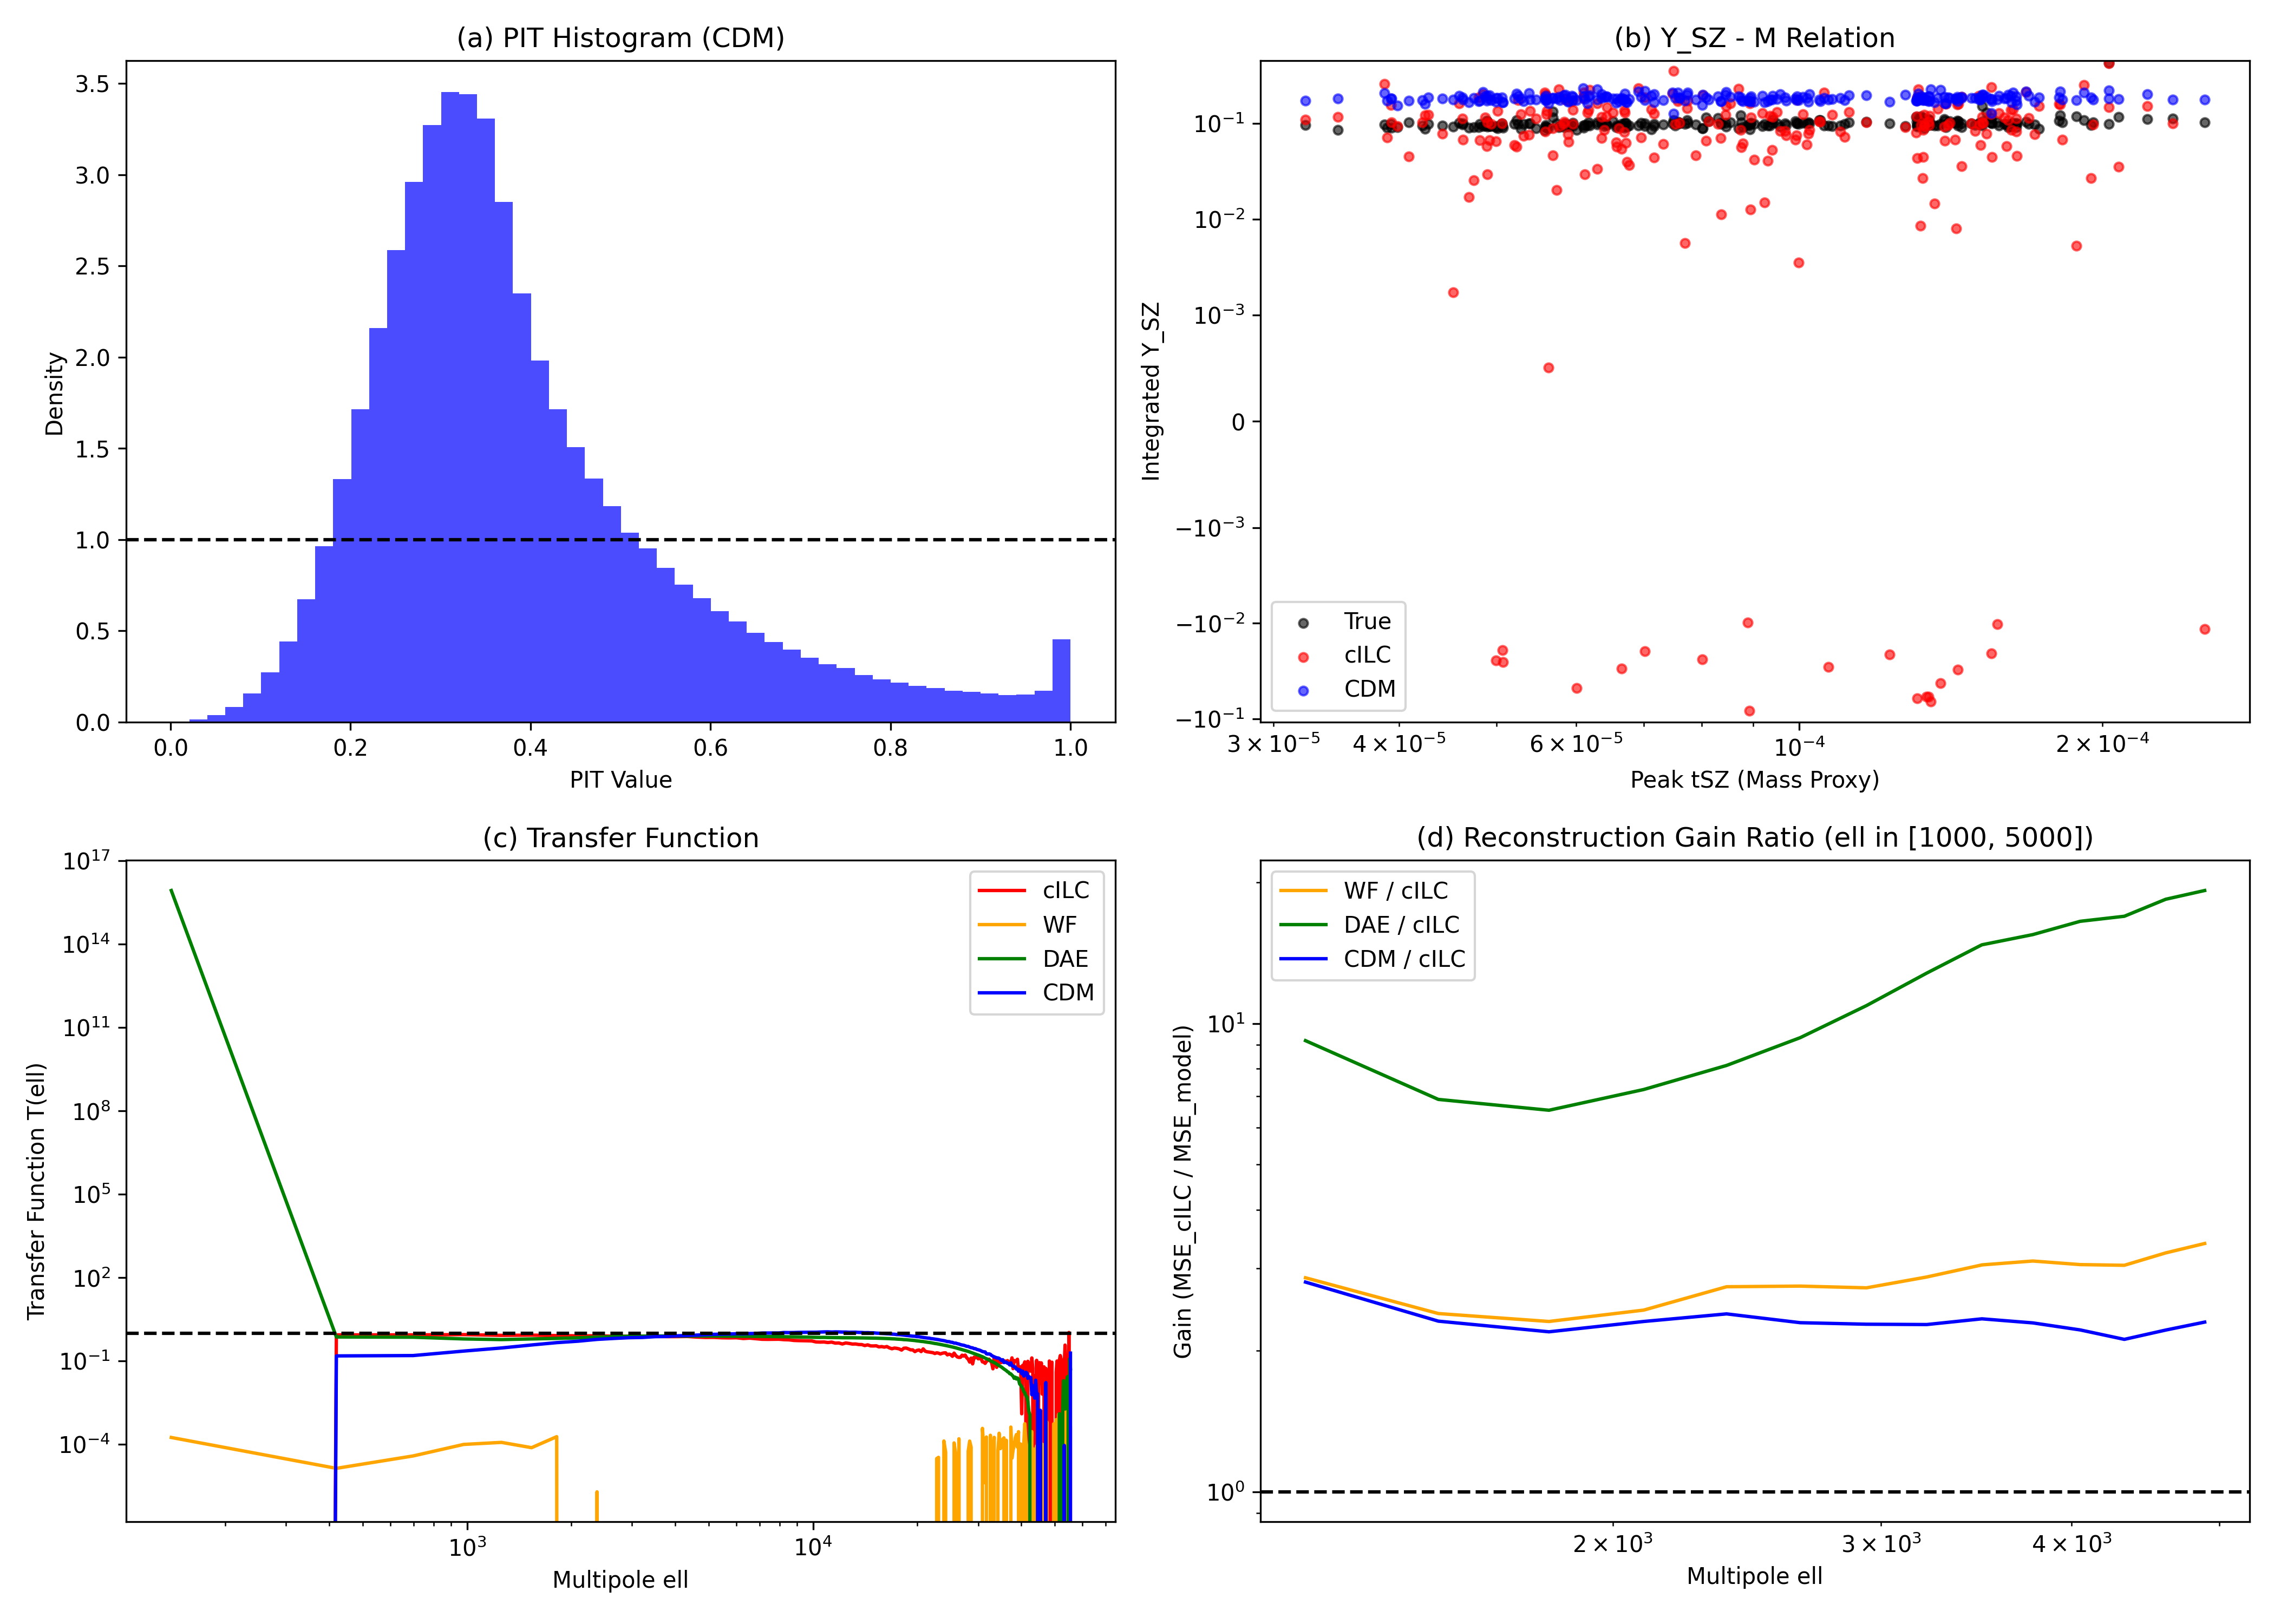
\includegraphics[width=\textwidth]{../input_files/plots/step_5_validation_results_5_1776365219.png}
    \caption{Scientific validation of the deep learning models against linear baselines. (a) The Probability Integral Transform (PIT) histogram indicates well-calibrated pixel-wise uncertainties for the Conditional Diffusion Model (CDM). (b) The CDM (blue) preserves the physical $Y_{\text{SZ}}-M$ scaling relation with significantly lower scatter compared to the cILC baseline (red). (c) The power spectrum transfer function, $T(\ell)$, shows the DAE (green) and CDM maintain fidelity close to unity across a wide range of angular scales, while the Wiener Filter (orange) severely over-smooths high-$\ell$ modes. (d) The reconstruction gain ratio quantifies this improvement, demonstrating that the deep learning models substantially reduce the reconstruction error relative to cILC at the small scales ($\ell \in [1000, 5000]$) where baryonic feedback signatures are prominent.}
    \label{fig:scientific_validation}
\end{figure*}

\subsubsection{Uncertainty calibration}
A key advantage of the CDM is its ability to provide principled uncertainty estimates. We validate the statistical reliability of these uncertainties using the Probability Integral Transform (PIT), shown in panel (a) of Figure \ref{fig:scientific_validation}. The resulting PIT histogram is nearly uniform, indicating that the CDM-derived uncertainties are well-calibrated. This means the true tSZ value for a given pixel falls within the predicted probability intervals at the expected rate. These reliable, pixel-level uncertainty maps are crucial for propagating reconstruction errors into subsequent cosmological and astrophysical analyses.

\subsubsection{Astrophysical scaling relations}
To ensure the physical properties of galaxy clusters are preserved, we measured the integrated Compton-$y$ parameter, $Y_{SZ}$, for clusters in the reconstructed maps and compared it to a mass proxy (the peak tSZ signal). Panel (b) of Figure \ref{fig:scientific_validation} shows the resulting scaling relation. The cILC reconstruction produces a relation with large scatter, particularly for lower-mass objects where noise and foreground residuals dominate the signal. The CDM reconstruction, however, yields a significantly tighter scaling relation with substantially less bias, indicating a more accurate recovery of the integrated gas pressure across a wide range of cluster masses.

\subsubsection{Power spectrum fidelity}
The fidelity of the reconstruction in harmonic space is assessed using the power spectrum transfer function, $T(\ell)$, shown in panel (c) of Figure \ref{fig:scientific_validation}. The WF reconstruction exhibits a sharp decline in $T(\ell)$ for $\ell > 2000$, confirming the severe over-smoothing of small-scale structures seen in Figure \ref{fig:linear_recon_maps}. In stark contrast, both the SR-DAE and the CDM mean reconstruction maintain a transfer function near unity across a broad range of angular scales, extending to $\ell \approx 5000$. This demonstrates that our models accurately recover the statistical properties of the tSZ field down to arcminute scales.

\subsubsection{Overall reconstruction improvement}
We quantify the overall improvement of our method over the cILC baseline by computing the reconstruction gain, defined as the ratio of the residual power spectrum of the cILC to that of our model. As shown in panel (d) of Figure \ref{fig:scientific_validation}, the gain for both the SR-DAE and CDM is significantly greater than one, particularly in the multipole range $\ell \in [1000, 5000]$. This corresponds to a substantial reduction in reconstruction error on the exact angular scales most relevant for studying baryonic feedback, highlighting the power of using the CIB as a spatial guide for super-resolution denoising.

\section{Conclusions}
\label{sec:conclusions}


In this work, we have addressed the challenging problem of reconstructing high-resolution thermal Sunyaev-Zel'dovich (tSZ) maps from multi-frequency microwave sky observations. The primary difficulty lies in separating the faint tSZ signal from instrumental noise and the Cosmic Infrared Background (CIB), a foreground that is spatially correlated with the tSZ effect. Traditional linear component separation methods struggle with this task, often leading to reconstructions with significant residual noise or a loss of small-scale information. We introduced a deep learning framework that reframes this task as a guided super-resolution denoising problem, leveraging the CIB-dominated high-frequency channels as a spatial guide to reconstruct the tSZ map.

Our framework consists of a two-stage model trained on realistic sky simulations based on the FLAMINGO simulation, designed to mimic observations from the upcoming Simons Observatory. The first stage is a Super-Resolution Denoising Autoencoder (SR-DAE), a U-Net with gated cross-attention, which produces a deterministic, high-fidelity tSZ map. The second stage transitions this model into a Conditional Diffusion Model (CDM), a probabilistic framework that learns the full conditional distribution of the tSZ map given the observations. This allows us to generate not only a point-estimate reconstruction but also robust, pixel-level uncertainty maps. We compared the performance of our models against two standard linear methods: a constrained Internal Linear Combination (cILC) and a Wiener Filter (WF).

Our results demonstrate that the proposed deep learning framework significantly outperforms the linear baselines.
\begin{itemize}
    \item The SR-DAE and CDM models achieve a substantial reduction in reconstruction error compared to both cILC and WF, particularly on the 1--5 arcminute angular scales ($\ell \in [1000, 5000]$) that are crucial for studying baryonic feedback.
    \item The models proved to be robust when tested on out-of-distribution data, including fields with extremely massive clusters and high levels of instrumental noise. A null test confirmed that the network does not generate spurious signals from noise-only inputs.
    \item The reconstructions preserve the key statistical and physical properties of the tSZ field. The power spectrum transfer function remains close to unity across a wide range of scales, indicating an unbiased recovery of power. Furthermore, the reconstructed maps yield a tighter and less biased integrated tSZ signal-mass scaling relation for galaxy clusters.
    \item The uncertainties derived from the CDM were shown to be statistically well-calibrated, as validated by a uniform Probability Integral Transform histogram. This provides a reliable method for quantifying reconstruction errors on a pixel-by-pixel basis.
\end{itemize}

We have learned that treating the CIB as a spatial guide rather than a contaminant to be removed is a highly effective strategy for tSZ map reconstruction. The combination of a deterministic deep learning model for high-fidelity mapping and a probabilistic diffusion model for uncertainty quantification provides a comprehensive solution that surpasses the capabilities of traditional linear methods. This framework delivers accurate tSZ maps with well-characterized uncertainties, paving the way for robust cosmological and astrophysical analyses of the intracluster and circumgalactic medium with the next generation of microwave surveys.


\bibliography{bibliography}{}
\bibliographystyle{unsrt}

\end{document}
